\documentclass{beamer}
\usepackage[final]{listings}
\usetheme{Madrid}
\usecolortheme{beaver}
\usefonttheme{professionalfonts}
\setbeamertemplate{footline}[page number]{}
\setbeamertemplate{navigation symbols}{}
\definecolor{burgundy}{rgb}{0.82, 0.1, 0.26}

\begin{document}
	
\title
{
	\texttt{bencherl}: A scalability benchmark suite for Erlang/OTP
}

\author
{
	Stavros Aronis\inst{1} \and
	Nikolaos Papaspyrou\inst{2} \and
	\textcolor{burgundy}{Katerina Roukounaki}\inst{2} \and
	Konstantinos Sagonas\inst{1,2} \and
	Yiannis Tsiouris\inst{2} \and
	Ioannis Venetis\inst{2}
}

\institute
{
	\inst{1}%
	Department of Information Technology, Uppsala University, Sweden
	\and
	\inst{2}%
	School of Electrical and Computer Engineering, National Technical University of Athens, Greece
}

\date
{Erlang Workshop 2012, Copenhagen}

\begin{frame}
	\titlepage
\end{frame}

\begin{frame}[t]{Motivation}
	\begin{block}{Frustrated Erlang programmer}
		I thought my Erlang program was {\bf 100\% parallelizable}, but when I made it parallel and ran it on a machine with {\bf N CPU cores}, I got a {\bf speedup} that was {\bf much lower than N}. Why?
	\end{block}
\end{frame}

\begin{frame}[t]{\texttt{bencherl}}
	\begin{itemize}
		\item runs benchmarks in an automatic way
		\item configurable extendable
examines 
can examine
can benchmark 
public available
tool
repository
examines 5 dimensions

	\end{itemize}
\end{frame}

\begin{frame}[t]{Architecture}
	\begin{center}
		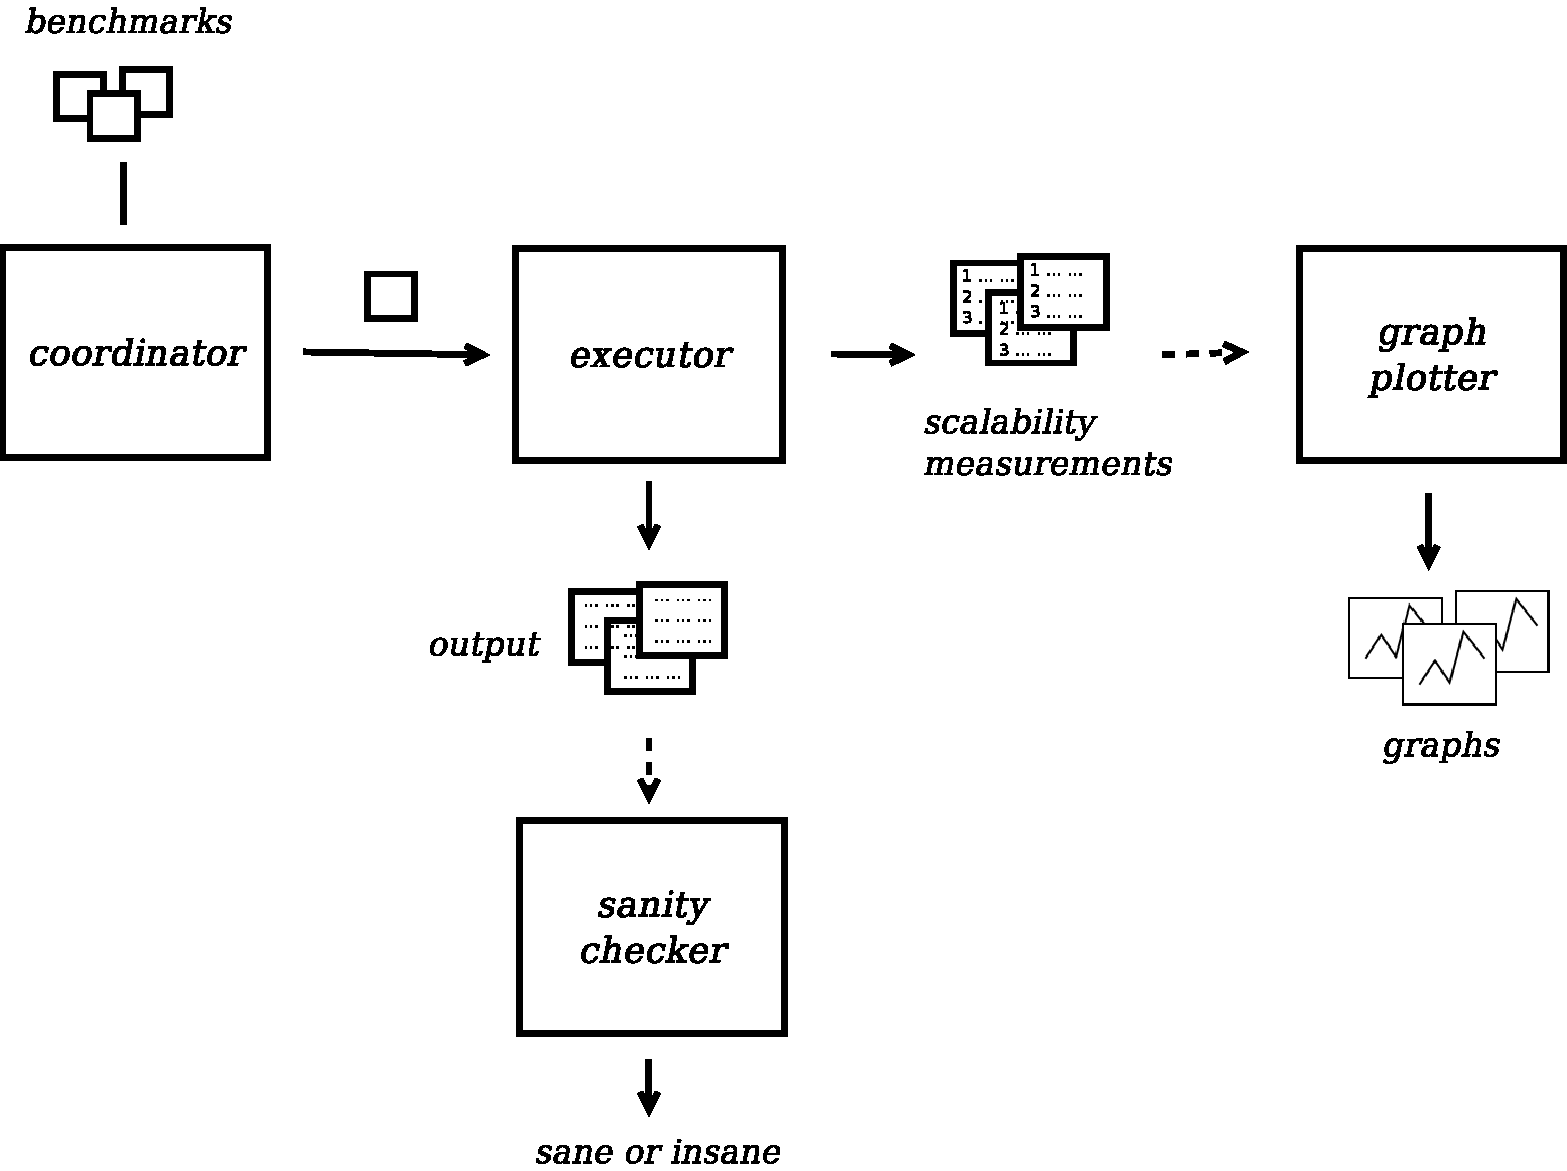
\includegraphics[width=0.8\linewidth]{figures/architecture.pdf}
	\end{center}
\end{frame}

\begin{frame}[t]{Coordinator}
	{\bf The module that coordinates everything during a \texttt{bencherl} run.}
	\begin{itemize}
		\item Determines the {\bf benchmarks} that should be executed
		\item Determines the {\bf runtime environments}, where each benchmark should be executed
		\item Sets up each runtime environment before a benchmark is executed in it
		\item Prepares instruction files for the \textcolor{burgundy}{executor}
		\item Performs any benchmark-specific pre- and post-execution actions
	\end{itemize}
\end{frame}

\begin{frame}[t]{Executor}
	{\bf The module that executes a particular benchmark in a particular runtime environment.}
	\begin{itemize}
		\item Receives detailed instructions from the \textcolor{burgundy}{executor} about what to do 
		\item Starts any necessary Erlang slave nodes
		\item Executes the benchmark in a new process
		\item Stops the Erlang slave nodes it started
		\item Makes sure that the output that the benchmark produced during its execution is written in an output file
		\item Makes sure that the measurements that are collected during the execution of the benchmark are written in a measument file 
			\begin{itemize}
				\item Uses \texttt{erlang:now/0} and \texttt{timer:diff/2}
			\end{itemize}
	\end{itemize}
\end{frame}

\begin{frame}[t]{Sanity checker}
	{\bf The module that checks whether all executions of a particular benchmark produced the same output.}
    \begin{itemize}
		\item Runs after a benchmark has executed in all desired runtime environments
		\item Examines the output that the benchmark produced in all runtime environments
		\item Decides whether the benchmark was successfully executed in all runtime environments
		\item Is based on the assumption that if a benchmark produces any output during its execution, then this output should be the same accross all runtime environments, where the benchmark was executed
			\begin{itemize}
				\item Uses \texttt{diff}
			\end{itemize}
    \end{itemize}
\end{frame}

\begin{frame}[t]{Graph plotter}
	{\bf The module that plots scalability graps based on the collected measurements.}
    \begin{itemize}
		\item Runs after a benchmark has executed in all desired runtime environments
		\item Processes the measurements that were collected during the execution of the benchmark
		\item Plots a set of scalability graphs
		\item Uses \texttt{Gnuplot}
    \end{itemize}
\end{frame}

\begin{frame}[t]{Scalability graphs}


\end{frame}

\begin{frame}[t]{Benchmarks}
	\texttt{bencherl} comes with an initial collection of benchmarks.
    \vspace{10pt}
	\begin{columns}[t]
		\begin{column}{0.45\textwidth}
			\begin{center}
			{\bf SYNTHETIC}
			\begin{columns}
				\begin{column}{0.45\textwidth}
					\begin{itemize}
						\item[] bang
						\item[] big
						\item[] ehb
						\item[] ets\_test
						\item[] genstress
						\item[] mbrot
					\end{itemize}
				\end{column}
				\begin{column}{0.45\textwidth}
					\begin{itemize}
						\item[] orbit\_int
						\item[] parallel
						\item[] pcmark
						\item[] ran
						\item[] serialmsg
						\item[] timer\_wheel
					\end{itemize}
				\end{column}
			\end{columns}
			\end{center}	
		\end{column}
        \begin{column}{0.45\textwidth}
			\begin{center}	
			{\bf REAL-WORLD}
			\begin{itemize}
				\item[] dialyzer\_bench
				\item[] scalaris\_bench
			\end{itemize}
			\end{center}
        \end{column}
	\end{columns}	
	\vspace{10pt}
	This collection can be enhanced in a number of simple steps.
\end{frame}

\begin{frame}[t]{Step 1: Add in \texttt{bencherl} everything that the benchmark needs for its execution.}
	\begin{itemize}
		\item The sources of the Erlang application that it benchmarks
		\item Any scripts to run before or after its execution
		\item Any data that it needs for its execution
	\end{itemize}
\end{frame}

\begin{frame}[fragile]{Step 2: Write the handler for the benchmark.}
	A benchmark handler is a standard Erlang module that exports two functions.
	\vspace{10pt}

	A function that returns the different argument sets that should be used for running a specific version of the benchmark:

	\begin{lstlisting}[basicstyle=\tiny,frame=single]
bench_args(Vrsn, Conf) -> Args
  when
    Vrsn :: 'short' | 'intermediate' | 'long',
    Conf :: [{Key :: atom(), Val :: term()}, ...],
    Args :: [[term()]].
	\end{lstlisting}

	A function that uses a specific argument set, specific Erlang slave nodes and specific configuration settings to run the benchmark:

    \begin{lstlisting}[basicstyle=\tiny,frame=single]
run(Args, Slaves, Conf) -> 'ok' | {'error', Reason}
  when
    Args   :: [term()],
    Slaves :: [node()],
    Conf   :: [{Key :: atom(), Val :: term()}, ...],
    Reason :: term().
	\end{lstlisting}

\end{frame}

\begin{frame}[fragile]{A benchmark handler example}

    \begin{lstlisting}[basicstyle=\tiny,frame=single]
-module(scalaris_bench).

-include_lib("kernel/include/inet.hrl").

-export([bench_args/2, run/3]).

bench_args(Version, Conf) ->
    {_,Cores} = lists:keyfind(number_of_cores, 1, Conf),
	[F1, F2, F3] = case Version of
		short -> [1, 1, 0.5];
		intermediate -> [1, 8, 0.5];
		long -> [1, 16, 0.5]
	end,
	[[T,I,V] || T <- [F1 * Cores], I <- [F2 * Cores], V <- [trunc(F3 * Cores)]].

run([T,I,V|_], _, _) ->
	{ok, N} = inet:gethostname(),
	{ok, #hostent{h_name=H}}=inet:gethostbyname(N),
	Node = "firstnode@" ++ H,
	rpc:block_call(list_to_atom(Node), api_vm, add_nodes, [V]),
	io:format("~p~n", [rpc:block_call(list_to_atom(Node), bench, quorum_read, [T,I])]),
	ok.
	\end{lstlisting}
\end{frame}

\begin{frame}{Experience \#1: Some benchmarks scale well.}
	\begin{center}
		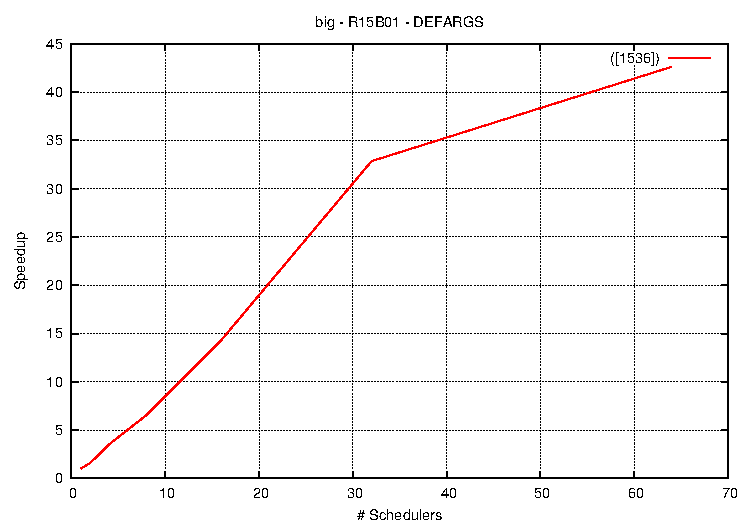
\includegraphics[width=0.8\linewidth]{figures/big-speedup-bulldozer.pdf}
	\end{center}
\end{frame}

\begin{frame}{Experience \#2: Some benchmarks scale do not scale as well on more than one nodes.}
    \begin{center}
        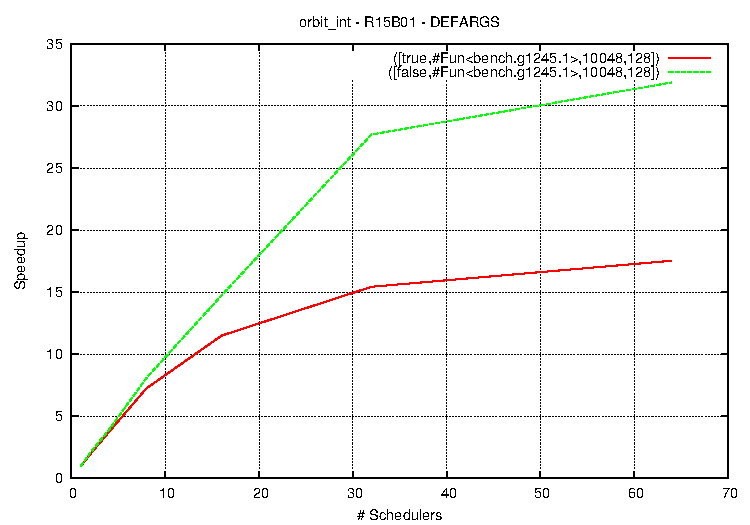
\includegraphics[width=0.45\linewidth]{figures/orbit_int_par-speedup-bulldozer.pdf}
        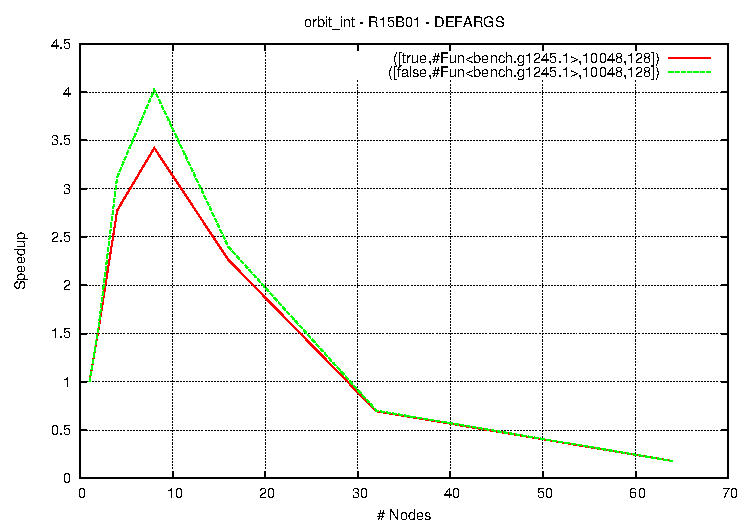
\includegraphics[width=0.45\linewidth]{figures/orbit_int_dist-speedup-bulldozer.pdf}
    \end{center}
\end{frame}

\begin{frame}{Experience \#3: Some benchmarks do not scale.}
    \begin{center}
        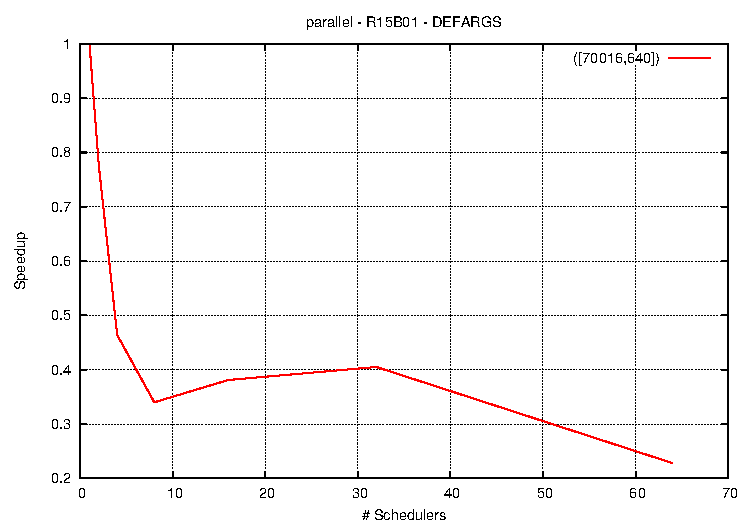
\includegraphics[width=0.8\linewidth]{figures/parallel-speedup-bulldozer.pdf}
    \end{center}
\end{frame}

\begin{frame}{Experience \#4: Some benchmarks scale better with specific runtime options.}
    \begin{center}
        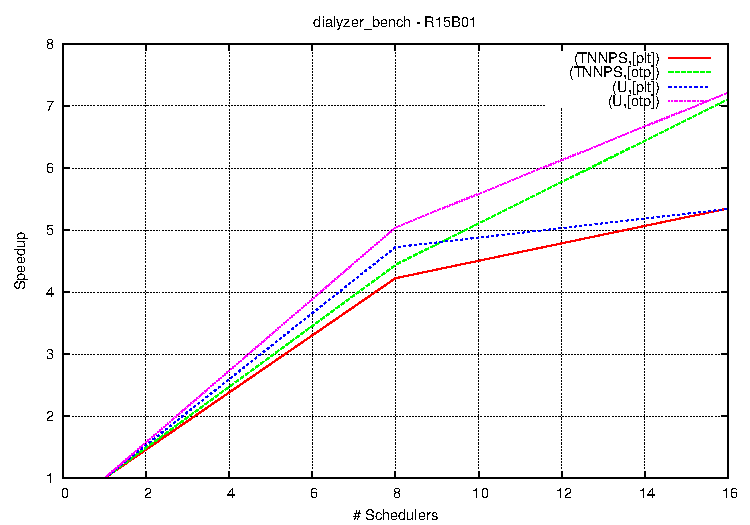
\includegraphics[width=0.8\linewidth]{figures/dialyzer_bench-speedup-bulldozer.pdf}
    \end{center}
\end{frame}

\begin{frame}{Experience \#5: Some benchmarks scale better with specific Erlang/OTP releases.}
    \begin{center}
        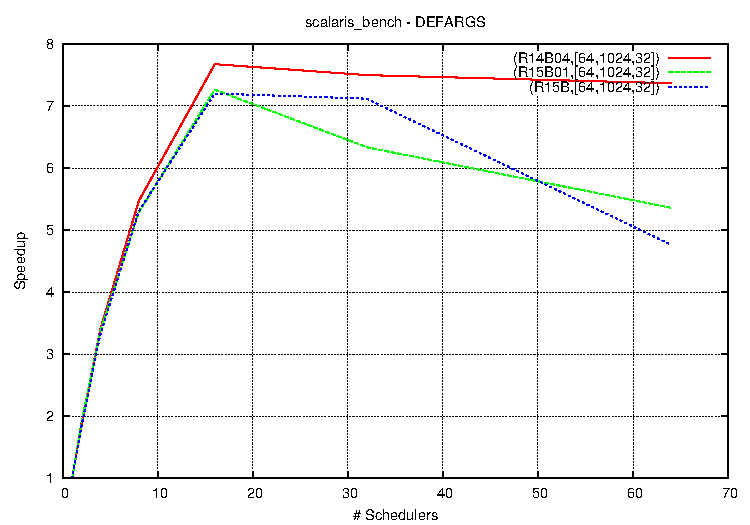
\includegraphics[width=0.8\linewidth]{figures/scalaris-speedup-bulldozer.pdf}
    \end{center}
\end{frame}

\begin{frame}[t]{Conclusions}
	\begin{itemize}
		\item 
	\end{itemize}
\end{frame}

\begin{frame}[t]{Future work}
\end{frame}

\begin{frame}
	\vspace{50pt}
	\begin{center}
	Thank you!
	\end{center}
\end{frame}

\end{document}

